
% % This section can go on section:4.2
Mongodb uses the concept of \textit{collections} and \textit{documents} to model data. Collections are the grouping of documents which generally have similar schema. Data has flexible schema where collections do not enforce document to structure rather requirements of our application. \todo{A collection is analogous to collection in XML database????} Documents are modeled as a data structure following the JSON format which actually store as BSON~\cite{bson}, a binary variant of JSON. \todo{what is BSON, diff btn JSON/BSON}. In Mongodb, there are two principle that allow application to represent documents and their relationship: \textit{reference} and \textit{embedded documents}. 
\todo{ need to change following image/json according to xmark data}
\begin{figure}
	\centering
	\subfigure[Reference document]{
		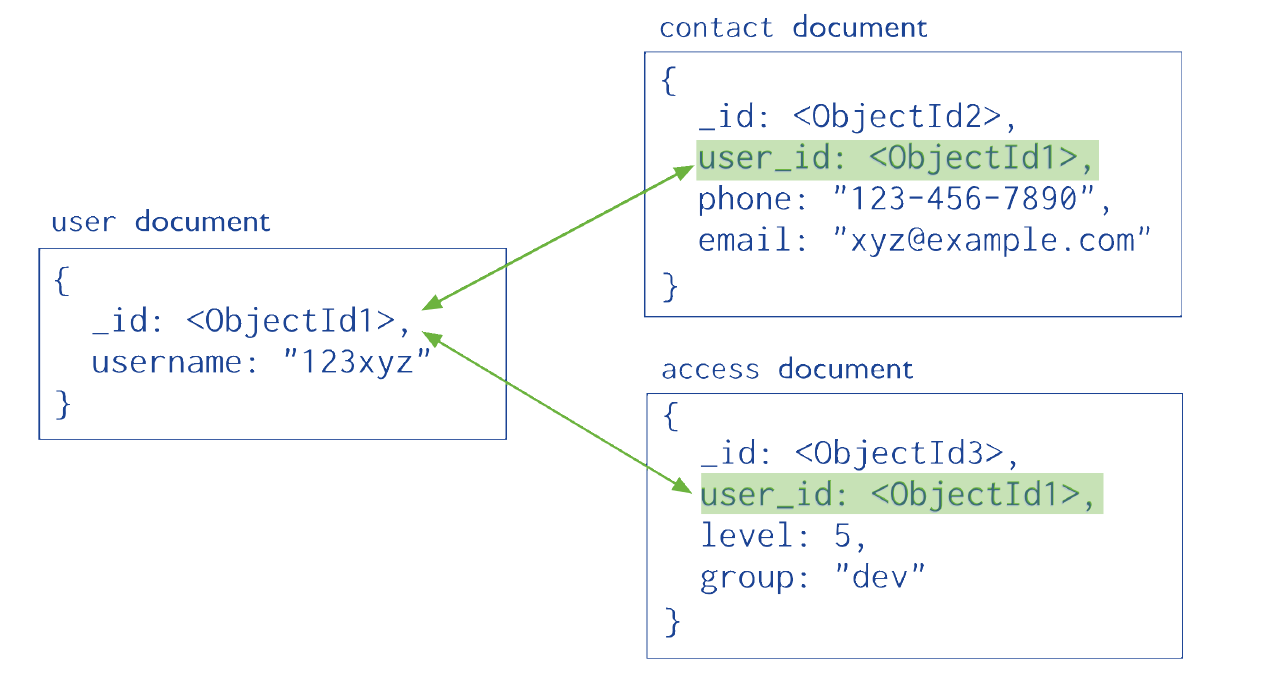
\includegraphics[width=0.44\textwidth]{img/mongodb-reference}
		%\caption{R-tree structure}
		\label{fig:mongodb-ref-doc}
	}
	\centering
	\subfigure[Embedded document]{
		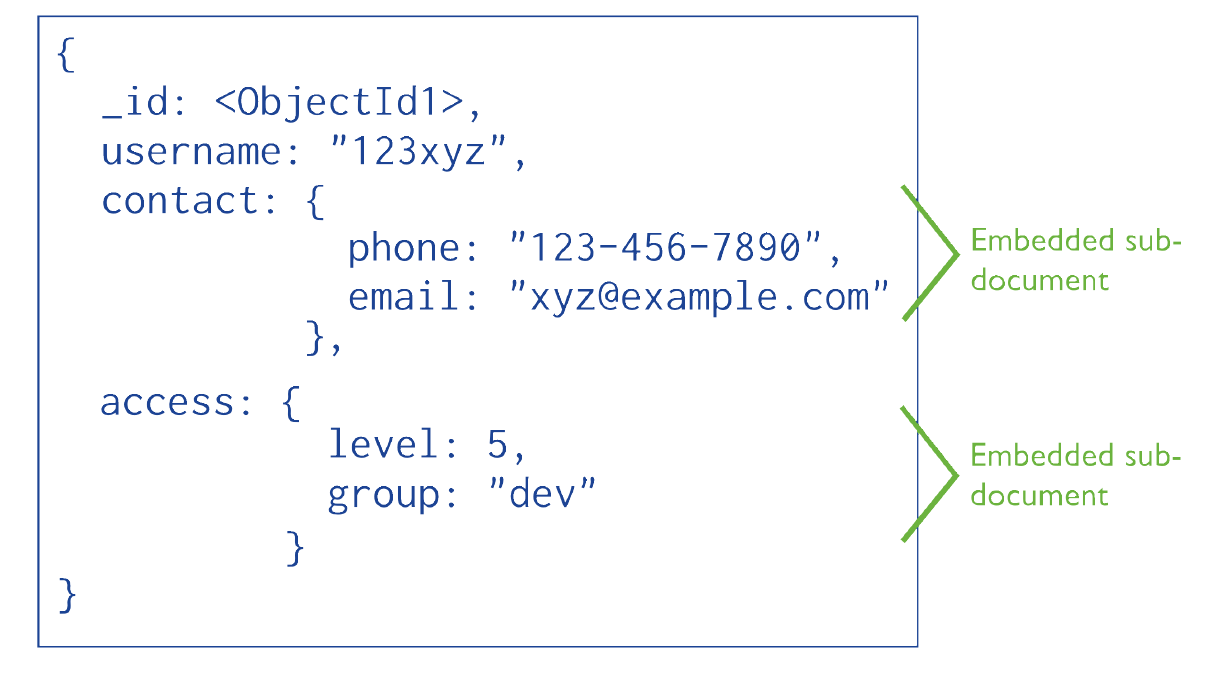
\includegraphics[width=0.44\textwidth]{img/mongodb-embedded}
		%\caption{R-tree}
		\label{fig:mongodb-emb-doc}
	}
	\caption{Mongodb document structure}
	\label{fig:mongodb-doc}
	 
\end{figure}

\paragraph{Reference}
	Reference stores the relationships between data by including links and references from one document to another as in  Figure~\ref{fig:mongodb-ref-doc}. The application can resolve these reference to access the related data\todo{Mongodb data model pg4}
\paragraph{Embedded}
	Embedded documents captures relationships between the data by storing related data in a single document structure. The documents in this method are structured as sub-documents\todo{...??} in the in the form of Array or/and Object~\cite{nosql/comparision}. 
	\label{mong-xmark-indexing}
\paragraph{Indexing} 
	Each document in Mongodb is uniquely identified by a field \textit{\_id} which is a primary index. Hence the collection is sorted by \textit{\_id} by default~\cite{nosql/comparision}. \todo{but note that this primary key index is not a clustered index in Database terms. I.e. the index entries only contains pointers to actual documents in the MongoDB data files. Documents are not physically stored in the order of \_id on disks.??  ::expand...page:9}
	

\subsubsubsection{XMARK in MongoDB}
	
	
	\iffalse\fi
	Monodbb's collections have a similar and related documents together that helps better indexing ultimately improve in performance. It will not worth to have single collection of whole XMark data as mentioned in \ref{xmark-nosql}. As we shown in Fig.~\ref{fig:xmark-schema}. we create each collection of each substructure in such a way that we will not lose data as well as most representation of xmark data. For Mongodb, the idea(?????) of in \ref{xmark-nosql} slightly change. Each \textit{doctype} represented as a collection. so we will have six collections and doctype is already represented by by the collections we don't need key/value of doctype in our document. For \textit{items},  \textit{regions} contains the name of region of each item as usual. 
	
	Finally as we mentioned in Indexing, the \textit{id} attribute of each these documents will be renamed to \textit{\_id} for default indexing. In case of \texttt{closed\_auctions} and \texttt{catgraph}, system will automatically generate \texttt{\_id} which is useless for our application.
\label{code:mongodb-person0}
\begin{fakeJSON}[label=json123,caption=Mongodb data representation of XMARk data]
{
	"_id": "person0",
	"name": "Kasidit Treweek",
	"emailaddress": "mailto:Treweek@cohera.com",
	"phone": "+0 (645) 43954155",
	"homepage": "http://www.cohera.com/~Treweek",
	"creditcard": "9941 9701 2489 4716",
	"profile": {
		"income": 20186.59,
		"interest": [{
			"category": "category251"
		}],
		"education": "Graduate School",
		"business": "No"
	}
	....
}
\end{fakeJSON} 
	
\subsubsubsection{Queries}
	coming soon ...
	
	
